\subsection{Monopole Antenna}\label{sec:monopole}
\subsubsection{Setup}
\FloatBarrier

\begin{figure}[htbp]
	\centering
	\hspace*{-0.0cm}
	\begin{subfigure}[t]{0.48\textwidth}
		\centering
		\includegraphics[height=8cm]{content/img/monopole_near_field}
		\caption{Electric near-field intensity}
		\label{fig:monopolenearfield}		
	\end{subfigure}
	\hfill
	\begin{subfigure}[t]{0.48\textwidth}
		
		\centering
		\raisebox{0.1cm}{\includegraphics[height=8cm]{content/img/monopole_antenna}}
		\caption{Geometry of monopole antenna}
		\label{fig:monopoleantenna}
	\end{subfigure}
	
	\caption{The geometrical aspects of the cylindrical monopole antenna, as implemented in the simulation model, with the respective electric near-field plot.}
	\label{fig:field_monopole_antenna}
\end{figure}

The monopole antenna is the simplest antenna capable of generating an electric dipole moment without any accompanying magnetic dipole moment. It is therefore analyzed first, to isolate the mechanisms behind electric dipole radiation from those of other antenna types discussed later in this chapter. As shown in \autoref{fig:monopoleantenna}, it is installed inside the TEM cell and connected to the feed point on the top wall, pointing towards the septum. The current flowing through the antenna is aligned with the electric field of the TEM mode, thereby producing an electric dipole moment according to \eqref{eqn:e_int_a} and \eqref{eqn:e_int_b}, which are further investigated in \cref{sec:eq_dip_mon}.

The antenna has a physical length of 5\,mm, making it electrically short across the entire frequency range of interest (up to 6\,GHz). Below 1.25\,GHz, the antenna is well approximated as an infinitesimal electric dipole, as discussed in \cref{sec:infinitesimal_electric_dipoles}. At higher frequencies, up to 6\,GHz, the finite current distribution along the wire demonstrated in \cref{sec:current_antenna_mon} becomes non-negligible, and the antenna is instead treated as a small electric dipole, as described in \cref{sec:small_electric_dipole}.

Numerically, the near-field distribution exhibits strong displacement currents near the feed point and at the antenna tip. To accurately resolve these localized field concentrations, the mesh element size is reduced in both regions, according to the procedure presented in \cref{sec:mesh}.

Because the electric dipole moment dominates the radiation mechanism, power transfer to the output ports occurs exclusively through displacement current coupling to the septum, as demonstrated in \cref{sec:el_small_antennas}. The induced septum current is analyzed in \cref{sec:sep_curr_mon} for two cases: the propagation of the TEM mode alone, and exclusive propagation of the TE\textsubscript{01} mode.

As an open-circuit structure, the monopole antenna exhibits capacitive behavior. Its effect on the frequency dependence of the feed voltage, current, and input impedance is discussed in \cref{sec:v_c_z_mon}. The output power produced by the antenna is compared against that of the equivalent dipole moments in \cref{sec:output_power_mon} to validate the simulation models.

Lastly, the theoretical framework and numerical results established in this thesis are combined in \cref{sec:monopole_eqc} to construct an equivalent circuit model, which represents the antenna, TEM cell and their coupling components. The circuit model provides an analytical description and deeper understanding of the driving coupling mechanisms between the TEM cell and the monopole antenna.

\subsubsection{Equivalent dipole moments}\label{sec:eq_dip_mon}

The equivalent electric and magnetic dipole moments, $\mathbf{m}_e$ and $\mathbf{m}_m$, are analytically derived using \eqref{eqn:ifa_me} and \eqref{eqn:ifa_mm}. The resulting $\mathbf{m}_e$ shown in \autoref{fig:dipolemomentsmonopolewide} increases approximately linearly over frequency, while the magnetic dipole moment $\mathbf{m}_m$ remains negligible throughout the investigated frequency range. This linear increase directly reflects the linear frequency dependence of the antenna current, as described by \eqref{eqn:e_int_a} and \eqref{eqn:e_int_b}, which relate the electric dipole moment to the antenna current. The frequency dependence of the current itself is shown in \autoref{fig:monopolefeedpointvoltagecurrent} and discussed further in \cref{sec:v_c_z_mon}.

\begin{figure}[htbp]
	\centering
	\includegraphics[width=1\linewidth]{content/img/dipole_moments_monopole_wide}
	\caption{The equivalent electric and magnetic dipole moments analytically calculated with \eqref{eqn:ifa_me} and \eqref{eqn:ifa_mm}. To enable direct comparison with the magnetic dipole moment, the electric dipole moment is weighted with the free space impedance $\eta_0$, as discussed in \cref{sec:prep_dip}.}
	\label{fig:dipolemomentsmonopolewide}
\end{figure}


%\begin{figure}[htbp]
%	\centering
%	\begin{subfigure}[b]{0.48\textwidth}
	%		\centering
	%		\includegraphics[width=1\linewidth]{content/img/dipole_moments_monopole.png}
	%		\caption{Equivalent dipole moments to model the monopole antenna.}
	%		\label{fig:dipole_moments_monopole}
	%	\end{subfigure}
%	\hfill
%	\begin{subfigure}[b]{0.48\textwidth}
	%		\centering
	%		\includegraphics[width=1\linewidth]{content/img/phase_shift_monopole}
	%		\caption{Phase shift of the power between the output ports produced by the monopole antenna.}
	%		\label{fig:phaseshiftmonopole}
	%	\end{subfigure}
%	
%	\caption{The equivalent dipole moments and the corresponding induced phase shift of the power between the output ports delivers information about the electric and magnetic coupling behavior of the monopole antenna.}
%	\label{fig:monopole_moments_phase}
%\end{figure}


\subsubsection{Feed voltage, current and impedance}\label{sec:v_c_z_mon}

The feedpoint voltage $V$ of the antenna, shown in \autoref{fig:monopolefeedpointvoltagecurrent}, remains largely constant over the investigated frequency range. Consequently, the voltage induced between the antenna and the septum is negligible, which is an observation consistent with the absence of a magnetic dipole moment $\mathbf{m}_m$ according to \autoref{eqn:m_v}. 

The feedpoint current $I$, shown in \autoref{fig:monopolefeedpointvoltagecurrent}, increases linearly with frequency. Since the monopole antenna has no return path, the entire current flows as displacement current, partially back toward the feedpoint as a reactive near-field component, and partially toward the septum, as is visible in \autoref{fig:monopolenearfield}. As described by \eqref{eqn:me_i}, $\mathbf{m}_e$ is directly proportional to this displacement current, which explains the observed linear increase of $\mathbf{m}_e$ with frequency. The constant feed voltage over frequency further supports this picture, since a frequency-independent voltage across a capacitive impedance must produce a displacement current that increases linearly with frequency. 

The capacitive nature of the antenna impedance is confirmed by the impedance plot in \autoref{fig:monopoleimp}, which shows a high impedance magnitude at low frequencies that decreases rapidly with increasing frequency. This behavior is characteristic of a capacitive impedance and is consistent with the prediction of \eqref{eqn:compl_power_inf_elec_dipole} and the discussion in \cref{sec:infinitesimal_electric_dipoles}.

\begin{figure}[htbp]
	\centering
	\begin{subfigure}[t]{0.48\textwidth}
		\centering
		\includegraphics[width=1\linewidth]{content/img/monopole_feedpoint_voltage_current}
		\caption{Voltage and current at feedpoint over frequency}
		\label{fig:monopolefeedpointvoltagecurrent}
	\end{subfigure}
	\hfill
	\begin{subfigure}[t]{0.48\textwidth}
		\centering
		\includegraphics[width=1\linewidth]{content/img/monopole_imp}
		\caption{Antenna impedance over frequency}
		\label{fig:monopoleimp}
	\end{subfigure}
	
	\caption{Magnitude of the voltage and current applied at the feedpoint of the monopole antenna over frequency, derived through the S-parameters with \eqref{eqn:iin} and \eqref{eqn:vin}, with the respective magnitude and phase of the antenna impedance over frequency, derived through the S-parameters with \eqref{eqn:za}.}
	\label{fig:monopoleimpvoltcurr}
\end{figure}

%The electric current present in the monopole antenna is aligned with the electric field $\mathbf{e}_\mathrm{TEM}^\pm$ of the dominant TEM mode present in the investigated frequency range. The electric dipole moment in y-direction suffices to model the antenna, because they align with the fields of the TEM mode.

\subsubsection{Current along antenna}\label{sec:current_antenna_mon}

Determining the distribution of the current along the monopole antenna validates the accuracy  of the numerical results and theoretical assumptions made previously. The current is numerically derived by integrating the magnetic field intensity $\mathbf{H}$ along a closed loop $C$ around the wire using Ampère's law,

\begin{equation}
	\oint_C \mathbf{H} \cdot d\mathbf{l'} = I.
	\label{eqn:ampere_law_fem}
\end{equation}

A fine mesh resolution is essential for obtaining accurate results from \eqref{eqn:ampere_law_fem}, as the obtained current values depend directly on the computed near-fields, which are particularly susceptible to numerical inaccuracies, as discussed in \cref{sec:mesh}. A coarse mesh causes non-linear behavior near the feedpoint at $0\,\mathrm{mm}$ in \autoref{fig:monopole_current_dist}, where significant displacement currents and numerical artifacts cause the current distribution to exhibit a steeper decline with non-physical oscillations.

The current distribution at $3\,\mathrm{GHz}$, shown in \autoref{fig:currentdistributionmonopole}, exhibits an approximately linear decrease from the feedpoint to zero at the antenna tip, consistent with the small electric dipole behavior described in \cref{sec:small_electric_dipole}. At $1\,\mathrm{MHz}$, shown in \autoref{fig:currentloopchargedistribution1mhz}, the variation in current along the antenna arm is negligible due to the antenna's small electrical size ($\ll\lambda/ 50$), and the current can be treated as constant, justifying the approximation of the monopole antenna as an infinitesimal electric dipole, as described in \cref{sec:infinitesimal_electric_dipoles}.

The electric dipole moment can be determined by integrating the current distribution along the monopole antenna according to \eqref{eqn:e_int_a} and \eqref{eqn:e_int_b}. At a frequency of 3\,GHz, this approach yields

\begin{equation}
	\mathbf{m}_\mathrm{e}(f=3\,\mathrm{GHz})=\int_{b/2-5\,\mathrm{mm}}^{b/2} I(y, f=3\,\mathrm{GHz})\,dy\, \mathbf{\hat{a}}_y = 85.69\,\upmu\mathrm{Am}\,\mathbf{\hat{a}}_y,
\end{equation}

which corresponds to $\mathbf{m}_e\cdot \eta_0=3.23\cdot 10^{-2} \cdot\,\mathrm{Vm}\,\mathbf{\hat{a}}_y$ when normalized by the free-space wave impedance $\eta_0$. This agrees well with the value of $\mathbf{m}_{e}$ in \autoref{fig:dipolemomentsmonopolewide} at 3\,GHz, therefore supporting the validity of \eqref{eqn:e_int_a} and \eqref{eqn:e_int_b}. 



\begin{figure}[htbp]
	\centering
	\begin{minipage}[t]{0.48\textwidth}
		\centering
		\centering
		\includegraphics[width=1\linewidth]{content/img/monopole_current_dist}
		\caption{Current distribution at $3\,\mathrm{GHz}$}
		\label{fig:currentdistributionmonopole}
		\hfill
	\end{minipage}
	\hfill
	\begin{minipage}[t]{0.48\textwidth}
		\centering
		\includegraphics[width=1\linewidth]{content/img/current_loop_charge_distribution_1MHz}
		\caption{Current distribution at $1\,\mathrm{MHz}$}
		\label{fig:currentloopchargedistribution1mhz}
	\end{minipage}
	\caption{The current distribution along the monopole antenna at $3\,\mathrm{GHz}$ and $1\,\mathrm{MHz}$.}
	\label{fig:monopole_current_dist}
\end{figure}

\FloatBarrier
\subsubsection{Current distribution on septum}\label{sec:sep_curr_mon}
\FloatBarrier

\begin{figure}[htbp]
	\centering
	\begin{subfigure}[b]{1\textwidth}
		\centering
		\includegraphics[width=1\linewidth]{content/img/monopole_surface_currents.png}
		\caption{Current surface density at 3\,GHz, where mostly the TEM mode propagates.}
		\label{fig:monopole_surface_currents}
	\end{subfigure}
	
	\vspace{1em} % Add vertical space between subfigures
	
	\begin{subfigure}[b]{1\textwidth}
		\centering
		\includegraphics[width=1\linewidth]{content/img/monopole_surface_currents_te01.png}
		\caption{Current surface density of only the TE\textsubscript{01}-mode at 3.3\,GHz with the TEM mode compensated.}
		\label{fig:monopole_surface_current_te01}
	\end{subfigure}
	
	\caption{Current surface densities at different frequencies, below and above the cut-off frequency of the TE\textsubscript{01}-mode.}
	\label{fig:surface-current}
\end{figure}

The monopole antenna transfers power to the output ports by inducing a current on the septum. This current is shown in \autoref{fig:monopole_surface_currents} at 3\,GHz. The current arrives at both output ports in phase, confirming the absence of a phase shift between the output port powers. This observation is consistent with the assumption that a pure electric dipole moment introduces no phase shift between the output port powers, as discussed in \cref{sec:equ-dip-mom}.

\autoref{fig:monopole_surface_current_te01} shows the septum surface current density at 3.3\,GHz, with the TEM mode suppressed at the output ports such that only the TE\textsubscript{01} mode propagates. The magnetic field of this mode has a $z$-component that increases gradually towards the cell walls, driving septum currents with an $x$-component that grows in magnitude toward the septum edge. Furthermore, the power induced at the two output ports exhibits a phase shift of $\pi$, a consequence of the TE\textsubscript{01} mode magnetic field being out of phase at the two ports, in contrast to the TEM mode, as explained in \cref{sec:equ-dip-mom}.

\subsubsection{Output power}\label{sec:output_power_mon}

The output power produced by the equivalent dipole moments $\mathbf{m}_e$ and $\mathbf{m}_m$ is compared to that of the monopole antenna in \autoref{fig:monopolemomentcomp}, showing agreement within a $\pm10\,$µW range. This demonstrates that the antenna is effectively represented by its equivalent dipole moments, further supporting the theoretical framework constructed in \cref{sec:el_small_antennas}, which connects electrically small antennas to their produced dipole moments.

The electric field $E^\pm_y$ at $x=0$, $y=b/4$, $z=\pm l/2$, shown in \autoref{fig:monopoleoutputpower}, increases linearly with frequency, consistent with the linearly increasing $\mathbf{m}_e$ magnitude and the resulting quadratic increase in output power. Furthermore, $E^\pm_y$ closely follows the frequency dependence predicted by \eqref{eqn:approx_e_field}, confirming the analytical approximation of the normalized electric field intensity derived in the preliminary theoretical discussion.

\begin{figure}[htbp]
	\centering
	\begin{subfigure}[t]{0.48\textwidth}
		\centering
		\includegraphics[width=1\linewidth]{content/img/monopole_output_power}
		\caption{$E_\mathrm{y}$ and power at output port}
		\label{fig:monopoleoutputpower}
	\end{subfigure}
	\hfill
	\begin{subfigure}[t]{0.48\textwidth}
		\centering
		\includegraphics[width=1\linewidth]{content/img/monopole_moment_comp}
		\caption{Comparison of output powers}
		\label{fig:monopolemomentcomp}
	\end{subfigure}
	\caption{Electric field component $E_\mathrm{y}$ at $x=0$, $y=b/4$, $z=\pm l/2$ and the corresponding output port power, computed from the S-parameters using \eqref{eqn:power_antenna}. The output power of the monopole antenna is compared against that produced by the equivalent dipole moments to validate the model.}
	\label{fig:monopole_power_comp}
\end{figure}

\FloatBarrier
\subsubsection{Equivalent circuit model}\label{sec:monopole_eqc}
\FloatBarrier

Equivalent circuit models of the antenna and the TEM cell are valuable tools 
for further analysis, as they allow the coupling mechanisms to be expressed in terms of measurable lumped circuit parameters. For the monopole antenna, an RLC series circuit for a short electric dipole \cite[p.~8]{Chu_1948} is applied, as demonstrated in \autoref{fig:eqc_simple_monopole}, where $R_A$, $L_A$ and $C_A$ represent the impedance behavior of the antenna.

\begin{figure}[h]
	\centering
	\resizebox{0.35\textwidth}{!}{
\begin{tikzpicture}
	% Capacitor in series
	\draw (7, 8) to[capacitor, l={$C_A$}] (8.75, 8);
	
	% Top horizontal wire connecting the two parallel branches
	\draw (8.75, 8) -- (10.75, 8);
	
	% Inductor branch (left, vertical) with its own ground
	\draw (8.75, 8) to[european inductor, l={$L_A$}] (8.75, 6);
	\node[ground] at (8.75, 6){};
	
	% Resistor branch (right, vertical) with its own ground
	\draw (10.75, 8) to[european resistor, l={$R_A$}] (10.75, 6);
	\node[ground] at (10.75, 6){};
	
	% Input wire and arrow
	\draw (7, 8) -- (6, 8);
	\draw[-latex] (5, 8.5) -- (6.75, 8.5);
	\node[shape=rectangle, minimum width=2.215cm, minimum height=0.965cm] 
	at (6.534, 8.75){} node[anchor=north west, align=left, 
	text width=1.827cm, inner sep=6pt] at (5.409, 9.25){$P_{in}$};
\end{tikzpicture}
	}
	\caption{Equivalent circuit for a short electric dipole models 
		the monopole antenna's behavior.}
	\label{fig:eqc_simple_monopole}
\end{figure}

Of primary concern for further analysis are $L_A$ and $C_A$, which are determined with the antenna model placed on a PEC surface in free space, as demonstrated in \autoref{fig:free-space-monopole}. The feed current $I_{in}$ is computed according to \eqref{eqn:iin}. The inductance and capacitance are derived according to 
\eqref{eqn:l_m_energy} and \eqref{eqn:c_e_energy}, which leads to 

\begin{subequations}
	\begin{equation}
		L_A = 2\frac{W_m}{I_{in}^2},
	\end{equation}
	\begin{equation}
		C_A = 2\frac{W_c}{V_{CA}^2}= \frac{I_{in}^2}{2\omega^2W_c},
	\end{equation}
\end{subequations}

where $V_{CA}=I_{in}/(j\omega C_A)$ denotes the voltage across the capacitor 
$C_A$. The resulting capacitance equals $C_A=98.36\,\mathrm{fF}$, and the inductance amounts to $L_A=1.14\,\mathrm{nH}$. The resistance $R_A$ generally represents conduction and radiation losses. However, only radiation losses are relevant here, as conduction losses are non-existent due to the use of PECs. The resistance $R_A$ can thereby be derived solely from the effective feed current $I_{in} / \sqrt{2}$ and the radiated power $P_{rad}$ along the radiation boundary, as expressed in 

\begin{equation}
	R_A = \frac{2P_{rad}}{I_{in}^2}.
\end{equation}

The resulting radiation resistance ranges from the milli-ohm range up to $3\,\Omega$ and increases quadratically with frequency.

\begin{figure}[h]
	\centering
	\includegraphics[width=0.7\linewidth]{content/img/free-space-monopole}
	\caption{Model of the monopole antenna connected to a feedpoint mounted 
		on a PEC surface with a side length of $\lambda/2$, where $\lambda$ 
		corresponds to the free-space wavelength of the solution frequency. This 
		configuration enables the investigation of the monopole antenna reactance 
		without influence of the TEM cell.}
	\label{fig:free-space-monopole}
\end{figure}

The antenna equivalent circuit is extended in \autoref{fig:full_circuit_monopole} 
to incorporate the TEM cell's electrical characteristics, represented by a total inductance $L_T = L_{T1} + L_{T2}$ and capacitance 
$C_T = C_{T1} + C_{T2}$, as derived in \cref{sec:tem_cell_model}. The components are split symmetrically ($L_{T1} = L_{T2}$ and $C_{T1} = C_{T2}$) to reflect the physical symmetry of the TEM cell. The source provides a constant input power $P_{in}=1\,\mathrm{W}$ and has a source resistance of $R_s=50\,\Omega$, representing the characteristic impedance of the feedpoint waveport in the simulation model.

The equivalent circuits of the antenna and the TEM cell are coupled via 
$C_k$, which models the displacement current coupling, and the mutual 
inductances $M_{A,T1}$ and $M_{A,T2}$, which account for coupling through 
induced voltages. The mutual inductances are incorporated in the overall schematic through inductor coupling, indicated by the dots next to the inductor symbols. Their relation to the branch voltages and currents is expressed by

\begin{equation}
	\mathbf{V} = j\omega \begin{bmatrix}
		L_{A}     & M_{A,T1} & M_{A,T2} \\
		M_{T1,A}  & L_{T1}   & 0 \\
		M_{T2,A}  & 0        & L_{T2}
	\end{bmatrix} \mathbf{I},
\end{equation}

where $\mathbf{I}=\left[ I_{LA}, I_{LT1}, I_{LT2} \right]^T$ denotes the current vector and $\mathbf{V}=\left[ V_{LA}, V_{LT1}, V_{LT2}  \right]^T$ the voltage vector, and the coupling is assumed to be reciprocal. The coupling elements $C_k$, $M_{A,T1}$, and $M_{A,T2}$ fully represent the power transfer to the TEM cell, rendering a separate radiation resistance $R_A$ redundant.

The key advantage of this approach is the direct derivation of the dipole moments from the circuit: $\mathbf{m}_m$ is obtained from the induced voltages across $L_{T1}$ and $L_{T2}$ in accordance with \eqref{eqn:m_v}, and $\mathbf{m}_e$ from the displacement current through $C_k$ according to \eqref{eqn:me_i}.

\begin{figure}[htbp]
	\centering
	\resizebox{\textwidth}{!}{%
\begin{tikzpicture}
	% Paths, nodes and wires:
	\node[shape=circle, draw, line width=1pt, minimum width=0.965cm]
	(N1) at (2.5, 9.5){} node[anchor=east] at (N1.west){$P_{in}$};
	\node[ground] at (2.5, 8){};
	\draw (2.5, 8) -- (2.5, 9);
	\draw (2.5, 10) -- (2.5, 11) -- (4, 11);
	\draw (4, 11) to[european resistor, l={$R_s$}] (6, 11);
	
	% C_A leads to the junction node
	\draw (6, 11) to[capacitor, l={$C_A$}] (8, 11);
	
	% Junction node where L_A taps off vertically
	\node[circ] at (8, 11){};
	
	% L_A placed vertically to ground (shunt element)
	\draw (8, 11) to[european inductor, l={$L_A$}] (8, 9);
	\node[ground] at (8, 9){};
	
	% Coupling dot on the right side, directly above the L_A label
	\node[circ] at (8.45, 10.5){};
	
	% Horizontal wire continues from junction to C_k
	\draw (8, 11) to[capacitor, l={$C_k$}] (14.5, 11);
	
	\node[shape=rectangle, draw, line width=1pt,
	dash pattern={on 4pt off 4pt}, minimum width=4.5cm,
	minimum height=5cm] at (8, 10.5){};
	\node[shape=rectangle, minimum width=5.215cm, minimum height=1.465cm]
	at (8.375, 13.5){} node[anchor=north west, align=left,
	text width=4.827cm, inner sep=6pt] at (5.75, 13.75){Antenna};
	
	\draw (14.5, 10) to[european inductor, l={$L_{T2}$}] (18, 10);
	\draw (14.5, 12) to[european inductor, l={$L_{T1}$}] (18, 12);
	\draw (14.5, 10) -| (14.5, 12);
	\node[circ] at (14.5, 11){};
	\draw (18, 10) to[capacitor, l={$C_{T2}$}] (18, 8);
	\draw (23, 10) to[european resistor, l={$R_2$}] (23, 8);
	\node[ground] at (18, 8){};
	\node[ground] at (20.5, 8){};
	\node[circ] at (18, 10){};
	\draw (18, 12) -- (22, 12);
	\draw (20.5, 10) to[capacitor, l={$C_{T1}$}] (20.5, 8);
	\node[ground] at (23, 8){};
	\draw (25.5, 10) to[european resistor, l={$R_1$}] (25.5, 8);
	\node[ground] at (25.5, 8){};
	\draw (22, 12) -- (24.5, 12);
	\draw (20.5, 10) -- (20.5, 12);
	\node[jump crossing] at (20.5, 10){};
	\draw (18, 10) -- (20.36, 10);
	\draw (20.64, 10) -- (23, 10);
	\draw (24.5, 12) -| (25.5, 10);
	\node[circ] at (20.5, 12){};
	\node[shape=rectangle, draw, line width=1pt,
	dash pattern={on 4pt off 4pt}, minimum width=7.965cm,
	minimum height=5.715cm] at (18, 9.875){};
	\node[shape=rectangle, minimum width=5.215cm, minimum height=1.465cm]
	at (16.375, 12.75){} node[anchor=north west, align=left,
	text width=4.827cm, inner sep=6pt] at (13.75, 13.5){TEM cell};
	\node[shape=rectangle, minimum width=2.715cm, minimum height=0.965cm]
	at (23.375, 10){} node[anchor=north west, align=left,
	text width=2.327cm, inner sep=6pt] at (22, 10.5){output port 2};
	\node[shape=rectangle, minimum width=2.715cm, minimum height=0.965cm]
	at (26.875, 10){} node[anchor=north west, align=left,
	text width=2.327cm, inner sep=6pt] at (25.5, 10.5){output port 1};
	\node[circ] at (15.75, 12.5){};
	\node[circ] at (16.75, 10.5){};
\end{tikzpicture}
	}
	\caption{Circuit representing the TEM cell and the monopole antenna, with 
		the additional components $C_k$ and $M_{A,T1}$, $M_{A,T2}$ modeling their 
		near-field coupling behavior.}
	\label{fig:full_circuit_monopole}
\end{figure}

The resulting $\mathbf{m}_e$ and $\mathbf{m}_m$ of the monopole antenna are depicted in \autoref{fig:eqc-dipoles-comp} and show quantitative agreement with the dipole moments derived by the simulator.

\begin{figure}[htbp]
	\centering
	\includegraphics[width=1\linewidth]{content/img/eqc-dipoles-comp}
	\caption{Equivalent dipole moments derived by the equivalent circuit compared to the previously derived dipole moments of the monopole antenna, shown in \autoref{fig:dipolemomentsmonopolewide}. The electric dipole moment $\mathbf{m}_e$ is weighted with $\eta_0$ for 
		comparison purposes.}
	\label{fig:eqc-dipoles-comp}
\end{figure}


\FloatBarrier




%\todo[inline]{idea: offset in z-direction, show surface current how it gets a pahse shift at waveports, and a magnetic dipole moment appears to be induced}
%\todo[inline]{idea: offset in x-direction, showing surface current and explaining the decrease in power transfer (normal E-field distribution)}

%If only the TEM mode propagates, only the y-component of an electric dipole moment and the x-component of a magnetic dipole moment generates output power, assuming they are centrally located ($x=0$, $y=b/4$, $z=0$). This is due to the magnetic field containing only an x-component $\mathbf{h}^\pm = h_x^\pm e^{\pm k_0 z}$, and the electric field only an y-component $\mathbf{e}^\pm = e_y^\pm e^{\pm k_0 z}$ at the center of the TEM cell. \todo{Sketch this situation. Also, $e^{\pm k_0 z}$ indicated that at z=0 the dipole moment is located. Consider this in all sketches}
%An offset of dipole moments or propagation of higher order modes lead to different field components of $\mathbf{h}^\pm$ and $\mathbf{e}^\pm$, and therefore to a change in coupling. These effects are investigated numerically in \autoref{sec:dipole_moments}.


\FloatBarrier
%\subsubsection{Electromagnetic energy in the TEM cell}
%\FloatBarrier
%
%The monopole antenna generates electromagnetic fields within the TEM cell, resulting in stored electromagnetic energy. The frequency-dependent electric energy is shown in \autoref{eqn:em_energy}. Its quadratic increase correlates with the output power in \autoref{fig:monopoleoutputpower}. The corresponding magnetic energy is several orders of magnitude smaller due to the capacitive behavior of the monopole antenna and is therefore neglected. From the stored electric energy, both the real and imaginary components of the power consumed by the antenna can be determined.
%
%Moreover, the effective inductance and capacitance of the monopole antenna inside the TEM cell can be derived from the magnetic and electric energy expressions given in \crefrange{eqn:l_m_energy}{eqn:c_e_energy}. Using the peak value of the electric energy shown in \autoref{fig:monopoleelecenergy}, the capacitance is estimated to be $C\approx108.55\,\mathrm{fF}$.
%
%\begin{figure}[htbp]
%	\centering
%	\includegraphics[width=1\linewidth]{content/img/monopole_elec_energy}
%	\caption{Electric energy determined by integrating the electric field over the TEM cell volume, using \autoref{eqn:em_energy}. }
%	\label{fig:monopoleelecenergy}
%\end{figure}

%\begin{figure}[htbp]
%	\centering
%	\begin{subfigure}[b]{0.48\textwidth}
	%	\centering
	%\includegraphics[width=1\linewidth]{content/img/monopole_magn_energy}
	%\caption{Magnetic energy determined with \autoref{eqn:em_energy}}
	%\label{fig:monopolemagenergy}
	%	\end{subfigure}
%	\hfill
%	\begin{subfigure}[b]{0.48\textwidth}
	%	\centering
	%\includegraphics[width=1\linewidth]{content/img/monopole_elec_energy}
	%\caption{Electric energy determined with \autoref{eqn:em_energy}}
	%\label{fig:monopoleelecenergy}
	%	\end{subfigure}
%	
%	\caption{Peak electromagnetic energy in the TEM cell generated by the monopole antenna}
%	\label{fig:monopole_em_energy}
%\end{figure}


\FloatBarrier